\section{Model Architecture \& Training Methodology}
\label{sec:model_architecture}

This section details Phase~3 of Deliverable~2, specifying the deep learning framework, backbone feature extractors, custom classification head, parameter distribution, objective functions, optimization strategies, and the systematic hyperparameter tuning protocol.

\subsection{Deep Learning Framework Selection}
\label{subsec:framework}

The deep learning pipeline is implemented using \textbf{PyTorch 2.x} and \textbf{Torchvision}. The choice of PyTorch over alternative frameworks (such as TensorFlow/Keras) was guided by four key architectural requirements:

\begin{enumerate}[leftmargin=*]
    \item \textbf{Dynamic Computational Graph and Execution Flexibility:} PyTorch's imperative execution model allows seamless layer-wise inspection, conditional gradient control during our progressive two-stage unfreezing schedule, and straightforward hooks for Grad-CAM explainability (\texttt{register\_forward\_hook} on intermediate feature maps).
    \item \textbf{High-Performance Hardware Acceleration:} Native support for mixed-precision arithmetic (\texttt{torch.cuda.amp.autocast} and \texttt{GradScaler}) substantially reduces GPU VRAM consumption on cloud NVIDIA Tesla T4 accelerators while accelerating matrix multiplications via Tensor Cores.
    \item \textbf{Standardized Pretrained Model Hub:} Torchvision provides audited, state-of-the-art ImageNet-1K pretrained weights (\texttt{ResNet50\_Weights.DEFAULT} and \texttt{EfficientNet\_B0\_Weights.DEFAULT}) with strictly documented normalization constants (\(\mu = [0.485, 0.456, 0.406]\), \(\sigma = [0.229, 0.224, 0.225]\)).
    \item \textbf{Deployment Modularity:} PyTorch facilitates clean extraction of model \texttt{state\_dict} checkpoints ($\sim$90--270\,MB) and straightforward conversion to TorchScript / ONNX for Phase~5 Streamlit web deployment.
\end{enumerate}

\subsection{Network Architecture \& Custom Classification Head}
\label{subsec:architecture}

Agricultural leaf disease detection presents unique computer vision challenges: distinguishing fine-grained textural symptoms (e.g., fungal rust pustules vs.\ bacterial leaf spots) while ignoring non-diagnostic background variations. We implement a modular architecture centered on \textbf{ResNet-50} as our primary deep feature extractor, with \textbf{EfficientNet-B0} available as a lightweight alternative for comparative benchmarking.

\subsubsection{Backbone Feature Extractor}
ResNet-50 utilizes residual learning with bottleneck blocks across four hierarchical stages. Each residual unit computes:
\begin{equation}
    \mathbf{y} = \mathcal{F}(\mathbf{x}, \{W_i\}) + \mathbf{x}
\end{equation}
where \(\mathbf{x}\) and \(\mathbf{y}\) are the input and output tensors, and \(\mathcal{F}\) represents the stacked $1\times 1$, $3\times 3$, and $1\times 1$ convolutions. The identity shortcut connections mitigate the vanishing gradient problem, allowing the extraction of both low-level morphological features (edges, color gradients in Stage 1) and complex semantic lesion patterns (Stage 4). 

The output of the final bottleneck block (\texttt{layer4[-1]}) has spatial dimensions $7 \times 7 \times 2048$ for an input image of $224 \times 224 \times 3$. This specific layer is explicitly designated as \texttt{model.target\_layer} to support gradient backpropagation for Grad-CAM saliency mapping.

\subsubsection{Feature Aggregation and Custom Head}
The standard 1000-class ImageNet fully connected layer is severed and replaced by our custom classification head:
\begin{enumerate}[leftmargin=*]
    \item \textbf{Adaptive Average Pooling:} An \texttt{AdaptiveAvgPool2d((1, 1))} collapses spatial dimensions, producing a compact $2048$-dimensional feature embedding vector independent of input resolution.
    \item \textbf{Dropout Regularization:} A dropout layer with probability $p = 0.30$ randomly zeros activations during training, preventing co-adaptation of deep representations and improving generalization to out-of-distribution field samples.
    \item \textbf{Linear Classification Layer:} A fully connected projection layer $\mathbf{W} \in \mathbb{R}^{2048 \times 38}$ with bias vector $\mathbf{b} \in \mathbb{R}^{38}$ maps deep latent features to unnormalized logit scores across all 38 plant health and disease classes:
    \begin{equation}
        \mathbf{z} = \mathbf{W}\mathbf{h} + \mathbf{b}, \quad \mathbf{z} \in \mathbb{R}^{38}
    \end{equation}
    where $\mathbf{h} \in \mathbb{R}^{2048}$ is the post-dropout embedding.
\end{enumerate}

\begin{figure}[t]
    \centering
    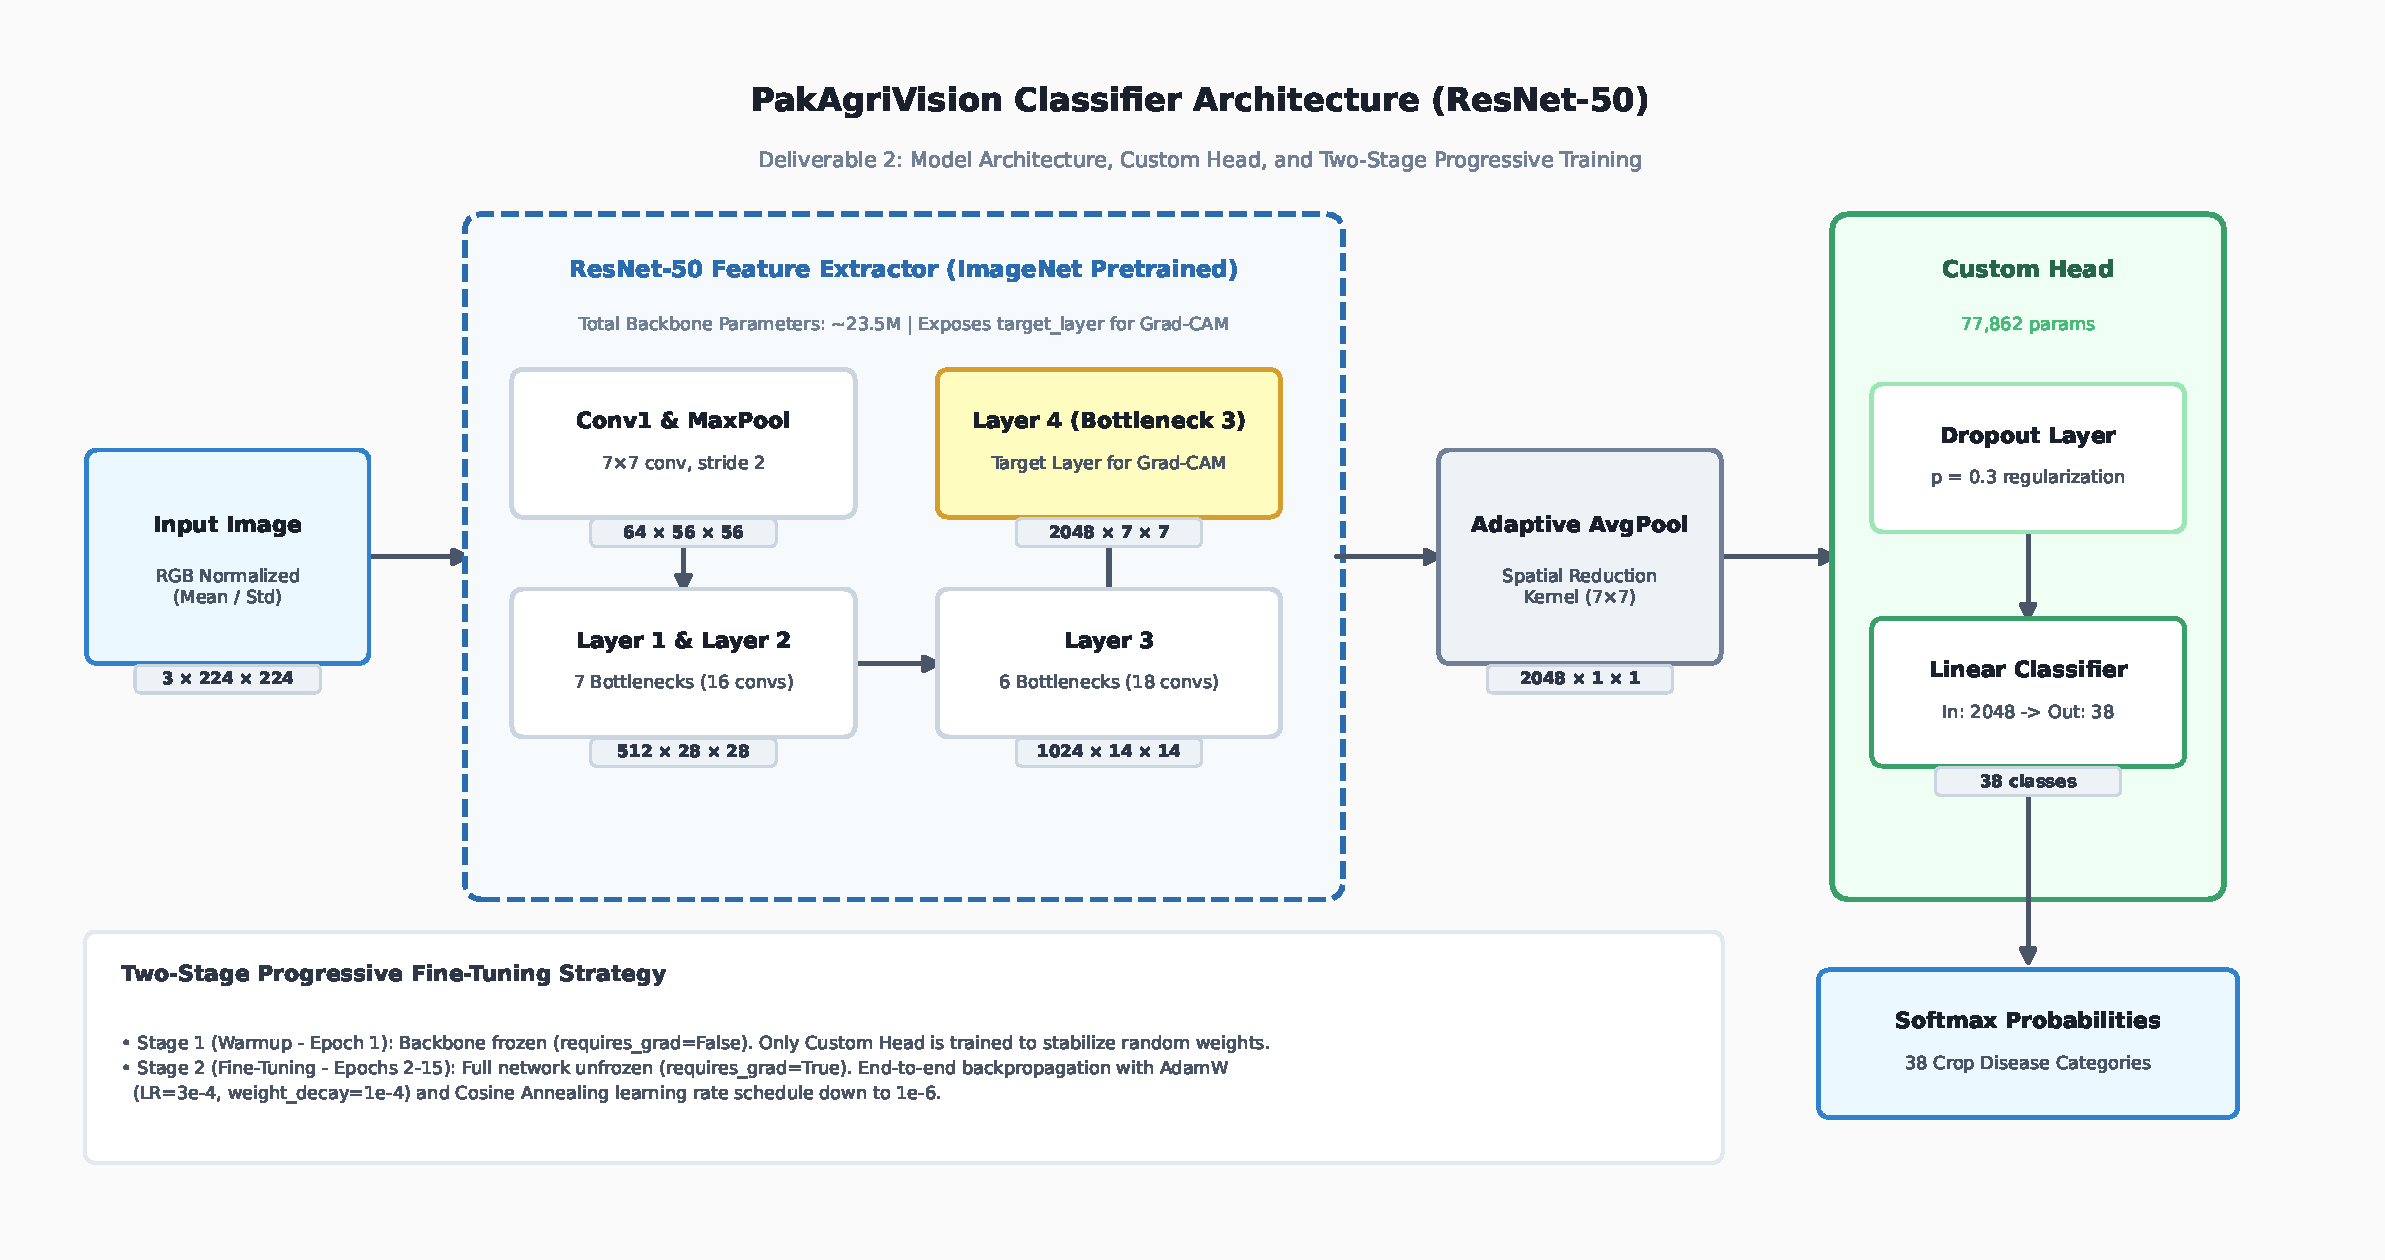
\includegraphics[width=\textwidth]{../../reports/figures/architecture.pdf}
    \caption{\textbf{PakAgriVision Model Architecture Pipeline.} Input leaf image ($3 \times 224 \times 224$) processed through the ResNet-50 residual backbone with bottleneck stages, adaptive average pooling, custom dropout ($p=0.3$), linear classification projection ($2048 \rightarrow 38$), and softmax normalization. The highlighted \texttt{layer4} bottleneck serves as the Grad-CAM explainability target layer.}
    \label{fig:model_architecture}
\end{figure}

\subsubsection{Parameter Counts and Resource Footprint}
Table~\ref{tab:parameter_counts} provides the exact parameter breakdown for our primary ResNet-50 architecture and the EfficientNet-B0 comparison baseline.

\begin{table}[h]
\centering
\small
\caption{\textbf{Model Parameter and Layer Breakdown.}}
\label{tab:parameter_counts}
\begin{tabular}{@{}lrrrr@{}}
\toprule
\textbf{Architecture} & \textbf{Backbone Params} & \textbf{Head Params} & \textbf{Total Params} & \textbf{Checkpoint Size} \\
\midrule
\textbf{ResNet-50 (Ours)} & 23,508,032 & 77,862 & \textbf{23,585,894} & $\sim$90.5\,MB (\texttt{state\_dict}) \\
\textbf{EfficientNet-B0} & 4,007,548 & 48,678 & \textbf{4,056,226} & $\sim$16.2\,MB (\texttt{state\_dict}) \\
\bottomrule
\end{tabular}
\end{table}

\subsection{Loss Function, Class Balancing \& Optimizer Strategy}
\label{subsec:loss_optim}

\subsubsection{Weighted Cross-Entropy Loss with Label Smoothing}
While our Phase~2 curation capped dominant classes at 1,000 images, minor agricultural diseases naturally have limited sample support in the training split (e.g., 152 samples in minority classes vs.\ 700 in capped classes). To ensure the model remains equally sensitive to rare, high-consequence crop infections, we implement class-weighted cross-entropy:
\begin{equation}
    \mathcal{L}_{\text{CE}}(\mathbf{z}, y) = - w_y \sum_{c=1}^{C} q_c \log \left( \frac{\exp(z_c)}{\sum_{j=1}^{C} \exp(z_j)} \right)
\end{equation}
where $w_y$ is the inverse frequency class weight for true class $y$ computed strictly on the training partition ($w_c \in \texttt{splits/class\_weights.json}$), and $q_c$ represents label-smoothed targets:
\begin{equation}
    q_c = (1 - \alpha) \cdot \mathbb{I}(c = y) + \frac{\alpha}{C}
\end{equation}
with smoothing parameter $\alpha \in [0.0, 0.10]$. Label smoothing prevents the model from generating overconfident, saturated logit predictions, significantly improving post-softmax calibration on uncertain field photographs.

\subsubsection{AdamW Optimizer \& Decoupled Weight Decay}
We select \textbf{AdamW} as our primary optimizer over standard SGD with momentum. AdamW decouples weight decay from the moving average gradient updates:
\begin{equation}
    \theta_{t+1} = \theta_t - \eta_t \frac{\hat{m}_t}{\sqrt{\hat{v}_t} + \epsilon} - \eta_t \lambda \theta_t
\end{equation}
where $\lambda = 10^{-4}$ is the weight decay rate, $\eta_t$ is the instantaneous learning rate, and $\hat{m}_t, \hat{v}_t$ are the bias-corrected first and second moment estimators. Decoupling ensures true $L_2$ regularization without distorting the adaptive gradient scaling.

\subsubsection{Two-Stage Progressive Fine-Tuning with Cosine Annealing}
Directly fine-tuning all layers simultaneously with a randomly initialized classification head can cause large, erratic gradient updates that destroy pretrained ImageNet feature detectors (catastrophic forgetting). We address this with a \textbf{Two-Stage Progressive Training Strategy}:

\begin{itemize}[leftmargin=*]
    \item \textbf{Stage 1: Head Warm-up (Epoch 1):} All backbone convolutional parameters are frozen via \texttt{set\_backbone\_trainable(model, False)} such that $\nabla_{\theta_{\text{backbone}}} \mathcal{L} = 0$. Only the randomly initialized weights of the custom head are optimized for one epoch with a linear learning rate warmup factor from $0.1 \times \eta_{\max}$ to $\eta_{\max} = 3 \times 10^{-4}$.
    \item \textbf{Stage 2: Full Fine-Tuning (Epochs 2--15):} The backbone is unfrozen (\texttt{set\_backbone\_trainable(model, True)}). All $23.5$\,M parameters are jointly fine-tuned using a \textbf{Cosine Annealing Schedule}:
    \begin{equation}
        \eta_t = \eta_{\min} + \frac{1}{2}(\eta_{\max} - \eta_{\min})\left(1 + \cos\left(\frac{t - t_{\text{warmup}}}{T_{\text{max}} - t_{\text{warmup}}}\pi\right)\right)
    \end{equation}
    where $\eta_{\min} = 10^{-6}$ and $T_{\text{max}} = 15$. This guarantees smooth learning rate decay toward zero, allowing fine convergence without manual step-decay tuning.
\end{itemize}

\subsection{Systematic Hyperparameter Tuning Protocol (13 Trials)}
\label{subsec:hyperparameter_tuning}

To justify every architectural and optimization choice on empirical evidence rather than heuristic defaults, we implemented a structured 13-trial grid divided into two distinct search phases:

\begin{itemize}[leftmargin=*]
    \item \textbf{Stage A (Architectural Backbone \& Learning Rate, Trials 1--6):} Explores the Cartesian product of backbones $\{\text{ResNet-50}, \text{EfficientNet-B0}\}$ across three learning rate orders of magnitude $\{10^{-3}, 3\times 10^{-4}, 10^{-4}\}$, holding batch size at 64 and dropout at 0.3.
    \item \textbf{Stage B (Regularization \& Capacity Ablation, Trials 7--13):} Takes the best-performing configuration from Stage~A and benchmarks variations in dropout rate ($0.0, 0.5$), batch size ($32, 128$), higher weight decay ($10^{-2}$), label smoothing ($0.10$), and unweighted loss.
\end{itemize}

\subsubsection{Efficiency Protocol}
To maximize GPU resource efficiency on free cloud accelerators, each tuning trial is trained on a **20\% stratified train subset** (\texttt{subset\_frac=0.20}, 4,437 images) for **4 epochs**, and evaluated on the full, uncompromised validation split (4,747 images) using Macro-F1. Table~\ref{tab:tuning_trials} displays the structured trials and records the completed Stage~A results.

\begin{table}[htbp]
\centering
\caption{\textbf{Systematic 13-Trial Hyperparameter Tuning Grid and Results.}}
\label{tab:tuning_trials}
\resizebox{\textwidth}{!}{%
\begin{tabular}{@{}cclccccccrr@{}}
\toprule
\textbf{ID} & \textbf{Stage} & \textbf{Backbone} & \textbf{LR} & \textbf{Batch} & \textbf{Drop} & \textbf{WD} & \textbf{Smooth} & \textbf{Weights} & \textbf{Val Acc} & \textbf{Val Macro-F1} \\
\midrule
1 & A & ResNet-50 & $1\times 10^{-3}$ & 64 & 0.3 & $1\times 10^{-4}$ & 0.0 & Yes & 96.08\% & 0.9605 \\
2 & A & ResNet-50 & $3\times 10^{-4}$ & 64 & 0.3 & $1\times 10^{-4}$ & 0.0 & Yes & \textbf{96.12\%} & \textbf{0.9606} \\
3 & A & ResNet-50 & $1\times 10^{-4}$ & 64 & 0.3 & $1\times 10^{-4}$ & 0.0 & Yes & -- & -- \\
4 & A & EfficientNet-B0 & $1\times 10^{-3}$ & 64 & 0.3 & $1\times 10^{-4}$ & 0.0 & Yes & -- & -- \\
5 & A & EfficientNet-B0 & $3\times 10^{-4}$ & 64 & 0.3 & $1\times 10^{-4}$ & 0.0 & Yes & -- & -- \\
6 & A & EfficientNet-B0 & $1\times 10^{-4}$ & 64 & 0.3 & $1\times 10^{-4}$ & 0.0 & Yes & -- & -- \\
\midrule
7 & B & ResNet-50 & $3\times 10^{-4}$ & 64 & 0.0 & $1\times 10^{-4}$ & 0.0 & Yes & -- & -- \\
8 & B & ResNet-50 & $3\times 10^{-4}$ & 64 & 0.5 & $1\times 10^{-4}$ & 0.0 & Yes & -- & -- \\
9 & B & ResNet-50 & $3\times 10^{-4}$ & 32 & 0.3 & $1\times 10^{-4}$ & 0.0 & Yes & -- & -- \\
10 & B & ResNet-50 & $3\times 10^{-4}$ & 128 & 0.3 & $1\times 10^{-4}$ & 0.0 & Yes & -- & -- \\
11 & B & ResNet-50 & $3\times 10^{-4}$ & 64 & 0.3 & $1\times 10^{-2}$ & 0.0 & Yes & -- & -- \\
12 & B & ResNet-50 & $3\times 10^{-4}$ & 64 & 0.3 & $1\times 10^{-4}$ & 0.1 & Yes & -- & -- \\
13 & B & ResNet-50 & $3\times 10^{-4}$ & 64 & 0.3 & $1\times 10^{-4}$ & 0.0 & No & -- & -- \\
\bottomrule
\end{tabular}%
}
\end{table}

